\section{Week 8}
General Observations:
\begin{itemize}
    \item The Mach number and speed of the flow decrease across a shock wave;
    \item Because the flow across shock waves is non-isentropic, the total pressure downstream of the shock is always less than the total pressure upstream of the shock; there is a loss of total pressure associated with a shock wave.
    \item Through an expansion fan, the Mach number increases, the static pressure decreases and the total pressure remains constant.
\end{itemize}
\Large \textbf{{\color{red}\underline{Normal Shocks}}}

\begin{itemize}
    \item Non-isentropic process
    \item Non-trivial solution for {\color{blue}compressible} flows:
    \begin{itemize}
        \item Density ratio:
        \begin{equation*}
            \frac{\rho_2}{\rho_1} = \frac{u_1}{u_2} = \frac{(\gamma + 1)M_1^2}{2+(\gamma - 1)M_1^2}
        \end{equation*}
        \item Pressure ratio:
        \begin{equation*}
            \frac{P_2}{P_1} = 1 + \frac{2 \gamma}{\gamma + 1} (M_1^2 - 1)
        \end{equation*}
        \item Temperature ratio:
        \begin{align*}
            \frac{T_2}{T_1} &= \left[ 1 + \frac{2\gamma}{\gamma + 1}(M_1^2 - 1) \right]\\
            &\cdot \frac{2+(\gamma - 1)M_1^2}{(\gamma + 1)M_1^2}
        \end{align*}
        \item Mach number ratio:
        \begin{equation*}
            M_2^2 = \frac{1+\frac{\gamma - 1}{2}M_1^2}{\gamma M_1^2 - \frac{\gamma - 1}{2}}
        \end{equation*}
        \item Entropy $s$ ratio
        \begin{align*}
            s_2 - s_1 &= c_p \ln\left(\left[1+\frac{2\gamma(M_1^2 - 1)}{\gamma+1}\right]\right. \\
            &\cdot \left. \frac{2+(\gamma-1)M_1^2}{(\gamma + 1)M_1^2}\right) \\
            &- R \ln\left( 1 + \frac{2\gamma}{\gamma + 1}(M_1^2 - 1) \right)
        \end{align*}
        Note that since $s_2 - s_1 \geq 0$, $\therefore M_1^2\geq 1$. Thus normal shock only occurs for supersonic flow.
    \end{itemize}
\end{itemize}

\large \textbf{\underline{Stagnation properties cross a normal shock}}

\begin{itemize}
    \item Non-isentropic processes across the shock:
    \begin{itemize}
        \item {\color{blue}Stagnation Pressure Change}
        \begin{equation*}
            \frac{P_{0,2}}{P_{0,1}} = e^{-\frac{(s_2-s_1)}{R}} \leq 1
        \end{equation*}
        \item {\color{blue}Stagnation Temperature} is constant across the normal shock
        \begin{equation*}
            T_{0,1} = T_{0,2}
        \end{equation*}
    \end{itemize}
\end{itemize}

\Large \textbf{{\color{red}\underline{Oblique Shocks}}}

Def: oblique shocks are waves occurred at concave corners. It is a {\color{red}non-isentropic} process.
\begin{figure}[H]
    \centering
    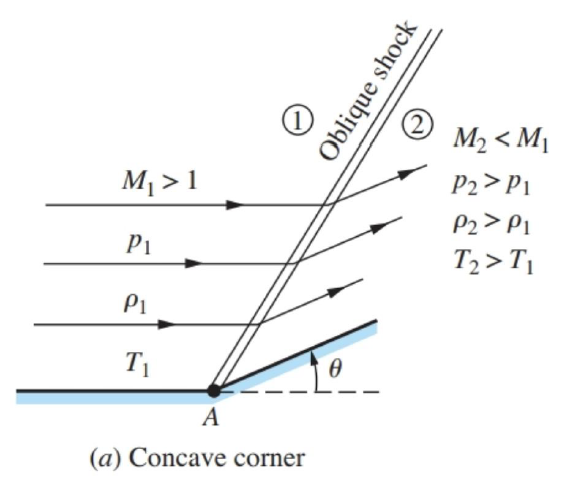
\includegraphics[width=1.0\linewidth]{images/oblique_shock_concave.png}
\end{figure}

Freebody Diagram:

\begin{figure}[H]
    \centering
    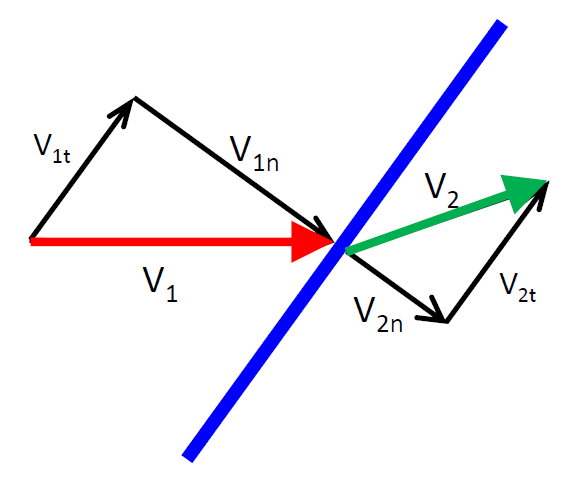
\includegraphics[width=1.0\linewidth]{images/oblique_shocks.png}
\end{figure}
\begin{itemize}
    \item Tangential component unchanged, $V_{1t} = V_{2t}$
    \item Normal component reduces, $V_{2n}<V_{1n}$
\end{itemize}

\textbf{{\color{blue}\underline{A Wedge Case}}}
\begin{itemize}
    \item {\color{red}Upstream of the shock:}
    \begin{figure}[H]
        \centering
        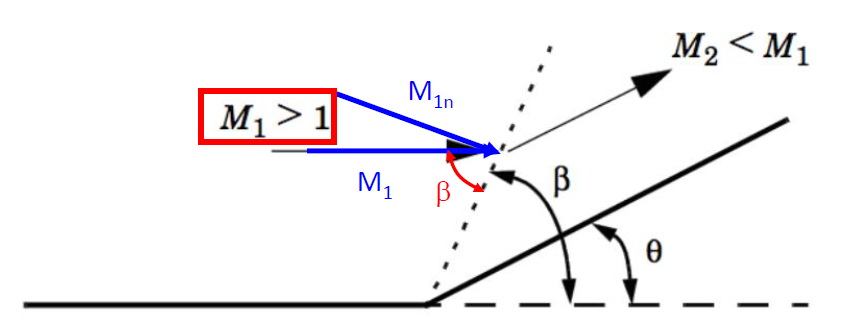
\includegraphics[width=1.0\linewidth]{images/oblique_shocks_upstream.png}
    \end{figure}
    \begin{equation*}
        M_1 = \frac{M_{1n}}{\sin(\beta)}
    \end{equation*}
    Since for a shock to form, it is required that $M_{1n}>1$. Thus, {\color{blue}$M_1 > 1$}. 
    \item $\theta$ is the \textbf{deflection/turning angle}, and $\beta$ is the \textbf{shock/wave angle}.
    
    \item {\color{red}Downstream of the shock:}
    \begin{figure}[H]
        \centering
        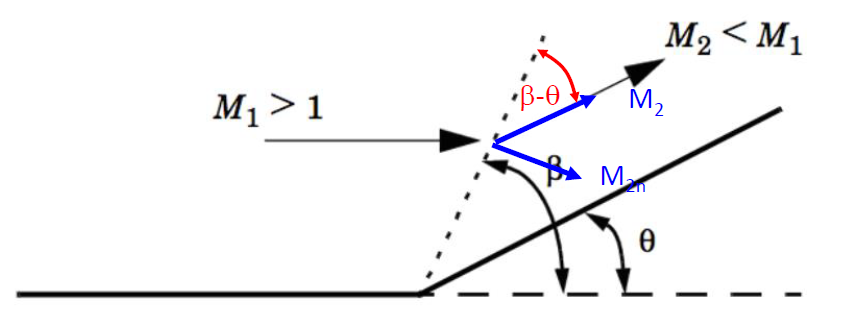
\includegraphics[width=1.0\linewidth]{images/oblique_shocks_downstream.png}
    \end{figure}
    \begin{equation*}
        M_2 = \frac{M_{2n}}{\sin(\beta - \theta)}
    \end{equation*}
    Flow after the shock must be subsonic, $M_{2n}<1$. However, {\color{blue}$M_2$ not necessarily $< 1$}.
    \item Ratios:
    \begin{itemize}
        \item Mach number ratio
        \begin{equation*}
            M_{n,2}^2 = \frac{1+[(\gamma - 1)/2]M_{n,1}^2}{\gamma M_{n,1}^2-(\gamma - 1)/2}
        \end{equation*}
        \item Density ratio
        \begin{equation*}
            \frac{\rho_2}{\rho_1} = \frac{(\gamma+1)M_{n,1}^2}{2+(\gamma-1)M_{n,1}^2}
        \end{equation*}
        \item Pressure ratio
        \begin{equation*}
            \frac{P_2}{P_1} = 1+ \frac{2\gamma}{\gamma + 1}(M_{n,1}^2 - 1)
        \end{equation*}
        \item Temperature ratio
        \begin{equation*}
            \frac{T_2}{T_1} = \frac{P_2}{P_1} \cdot \frac{\rho_1}{\rho_2}
        \end{equation*}
        \item Relation between $\theta$, $\beta$, $M$
        \begin{figure}[H]
            \centering
            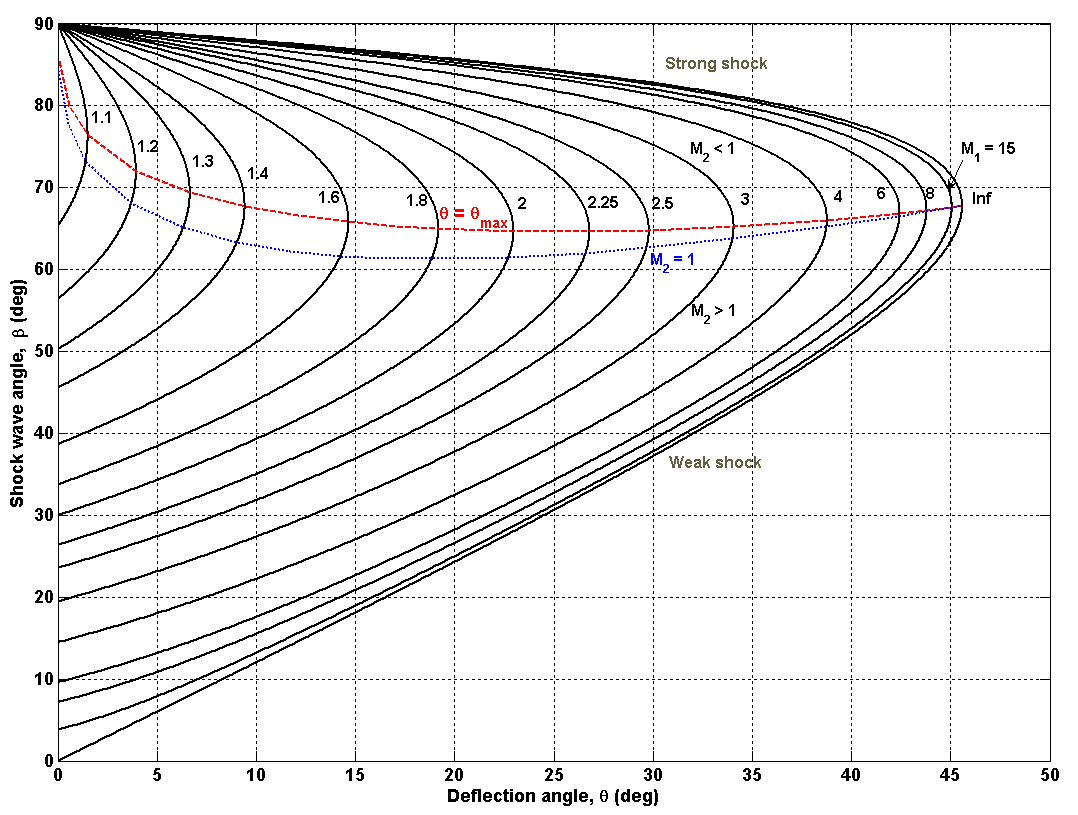
\includegraphics[width=1.0\linewidth]{images/angle-mach-relation.png}
        \end{figure}
        \begin{equation*}
            \tan(\theta) = 2\cot(\beta)\frac{\left(M_1^2\sin^2(\beta)\right)-1}{M_1^2 \left(\gamma + \cos(2\beta)\right)+2}
        \end{equation*}
        \item When $\theta = 0 ^{\circ}$, then $\beta = 90 ^{\circ} \rightarrow$ the normal shock solution.
        \item For every $\theta$ there are two solutions for $\beta$: the \textbf{weak shock} (smaller value of $\beta$) and the \textbf{strong shock} (larger value of $\beta$) - {\color{blue}the weak shock almost always prevails.}
        \begin{figure}[H]
            \centering
            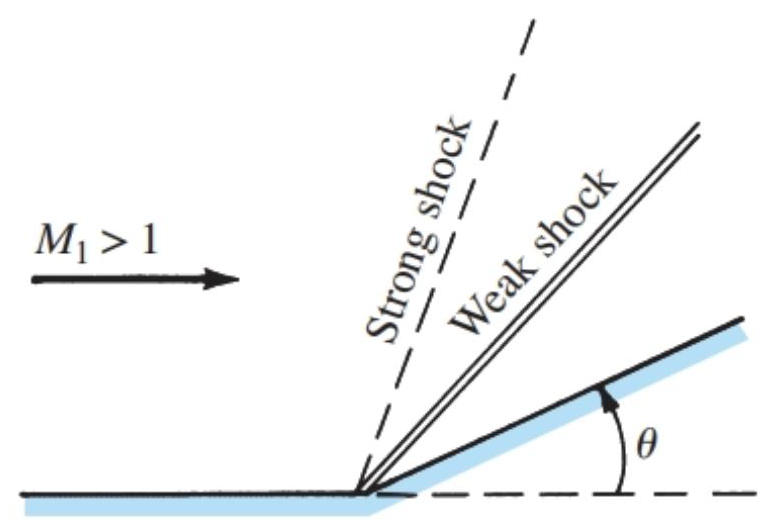
\includegraphics[width=0.8\linewidth]{images/weak_shock.png}
        \end{figure}
    \end{itemize}
\end{itemize}

\textbf{{\color{blue}\underline{Expansion Waves}}}

Def: expansion waves occurred at convex corners. It is a {\color{red}isentropic} process.
\begin{figure}[H]
    \centering
    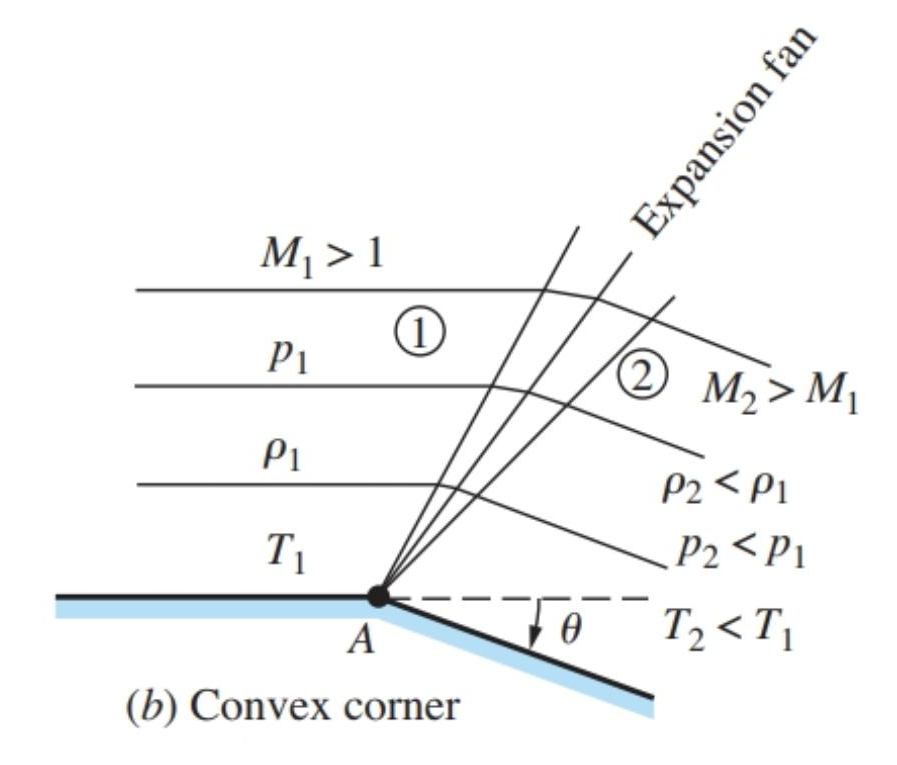
\includegraphics[width=1.0\linewidth]{images/expansion_wave_convex.png}
\end{figure}

\textbf{\large {\color{red}\underline{Expansion Fan}}}

\begin{itemize}
    \item The flow through the expansion fan is {\color{blue}ISENTROPIC} (thus, $T_{0,2}=T_{0,1}$ and $P_{0,2}=P_{0,1}$)
    \item Prandtl-Meyer Function (function of the incoming Mach number)
    \begin{align*}
        v(M) &= \sqrt{\frac{\gamma+1}{\gamma-1}}\tan^{-1}\left(\sqrt{\frac{\gamma-1}{\gamma+1}(M^2-1)}\right) \\
        &- \tan^{-1}\left(\sqrt{M^2-1}\right)
    \end{align*}
    $v(M)$ is also known as the \textbf{P-M angle}.
    \item Upstream-Downstream relation:
    \begin{equation*}
        \theta = v(M_2) - v(M_1)
    \end{equation*}
    \begin{figure}[H]
        \centering
        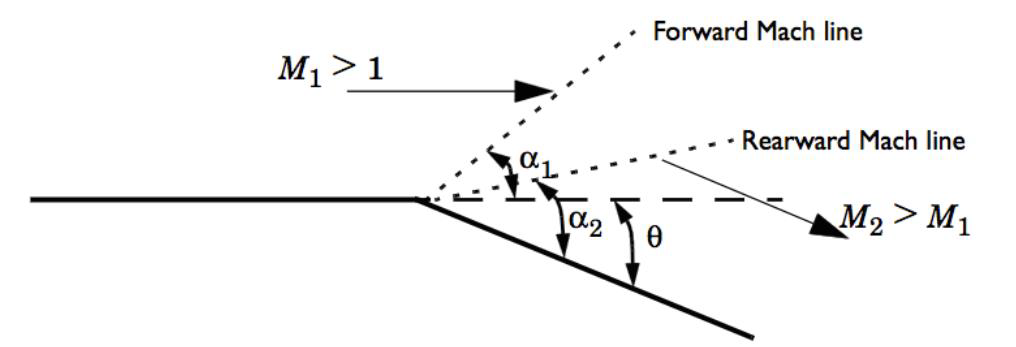
\includegraphics[width=1.0\linewidth]{images/expansion_wave_up_downstream.png}
    \end{figure}
    In exams, use the 'Isentropic Flow Relations' in this \href{http://www.dept.aoe.vt.edu/~devenpor/aoe3114/calc.html}{\color{blue}\underline{Online Calculator}\color{black}} to check P-M angle and $M_2$.
    \begin{itemize}
        \item \textbf{Mach angles} $\alpha_1$ and $\alpha_2$ (also written as $\mu_1$ and $\mu_2$)
        \begin{align*}
            \alpha_1 = \mu_1 &= \sin^{-1}\left(\frac{1}{M_1}\right) \\
            \alpha_2 = \mu_2 &= \sin^{-1}\left(\frac{1}{M_2}\right)
        \end{align*}
    \end{itemize}
    \item Ratios (use isentropic relations)
    \begin{itemize}
        \item Stagnation pressure $P_0$ is {\color{blue}unchanged}
        \item Pressure ratio:
        \begin{equation*}
            \frac{P_2}{P_1} = \left(\frac{1+\frac{\gamma-1}{2}M_1^2}{1+\frac{\gamma-1}{2}M_2^2}\right)^{\frac{\gamma}{\gamma-1}} = 0.6
        \end{equation*}
        \item Temperature ratio:
        \begin{equation*}
            \frac{T_2}{T_1} = \left(\frac{1+\frac{\gamma-1}{2}M_1^2}{1+\frac{\gamma-1}{2}M_2^2}\right)= 0.86
        \end{equation*}
        \item Density ratio:
        \begin{equation*}
            \frac{\rho_2}{\rho_1} = \left(\frac{1+\frac{\gamma-1}{2}M_1^2}{1+\frac{\gamma-1}{2}M_2^2}\right)^{\frac{1}{\gamma-1}}= 0.69
        \end{equation*}
    \end{itemize}
\end{itemize}

\large \textbf{\underline{{\color{red}Pitot-Static Tubes}}}
\begin{figure}[H]
    \centering
    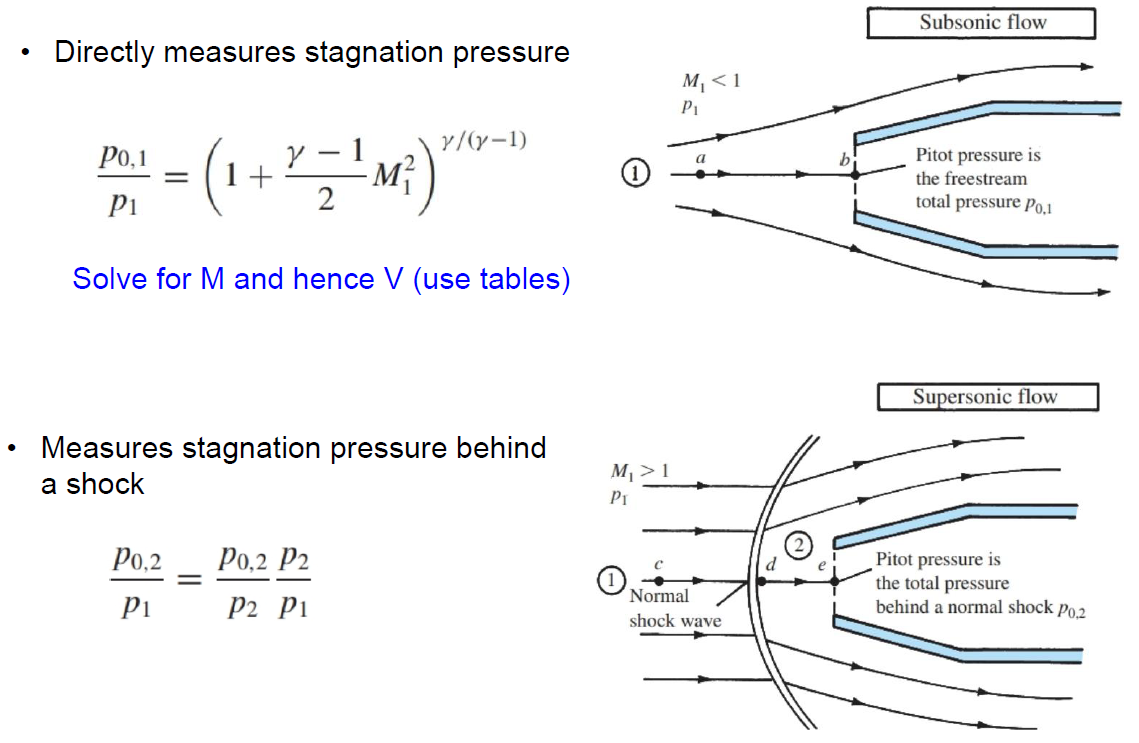
\includegraphics[width=1.0\linewidth]{images/Pitot_static_tubes.png}
\end{figure}

\large \textbf{\underline{{\color{red}Lift and Drag}}}
\begin{figure}[H]
    \centering
    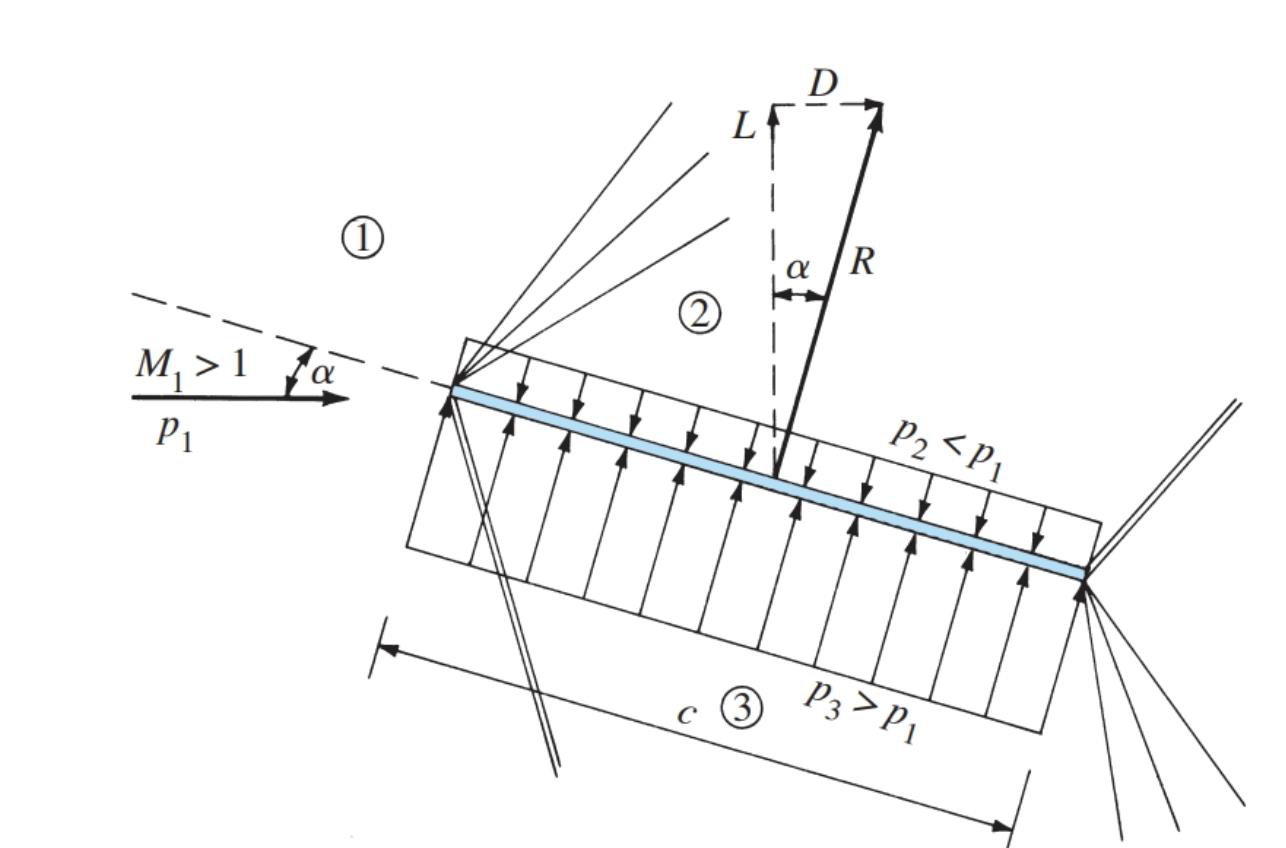
\includegraphics[width=1.0\linewidth]{images/Compressible_Aerodynamics.png}
\end{figure}

\begin{align*}
    R &= (p_3 - p_2 ) \cdot c \\
    L &= (p_3 - p_2 ) \cdot c \cdot \cos(\alpha) \\
    D &= (p_3 - p_2 ) \cdot c \cdot \sin(\alpha)
\end{align*}

\begin{itemize}
    \item Coefficient of Lift:
    \begin{align*}
        c_l &= \frac{L}{\frac{1}{2}\gamma P_1 M_1^2 S} \\
        \text{where } S &= c \times 1
    \end{align*}
    Note that S = chord length $\times$ unit depth. For 2D case, the depth is unity.
    \item Coefficient of Drag:
    \begin{equation*}
        c_d = \frac{D}{\frac{1}{2}\gamma P_1 M_1^2 S}
    \end{equation*}
\end{itemize}